% Options for packages loaded elsewhere
% Options for packages loaded elsewhere
\PassOptionsToPackage{unicode}{hyperref}
\PassOptionsToPackage{hyphens}{url}
%
\documentclass[
  ignorenonframetext,
  aspectratio=169,
  russian,
]{beamer}
\newif\ifbibliography
\usepackage{pgfpages}
\setbeamertemplate{caption}[numbered]
\setbeamertemplate{caption label separator}{: }
\setbeamercolor{caption name}{fg=normal text.fg}
\beamertemplatenavigationsymbolshorizontal
% Prevent slide breaks in the middle of a paragraph
\widowpenalties 1 10000
\raggedbottom
\AtBeginPart{
  \frame{\partpage}
}
\AtBeginSection{
  \ifbibliography
  \else
    \frame{\sectionpage}
  \fi
}
\AtBeginSubsection{
  \frame{\subsectionpage}
}
\usepackage{iftex}
\ifPDFTeX
  \usepackage[T1]{fontenc}
  \usepackage[utf8]{inputenc}
  \usepackage{textcomp} % provide euro and other symbols
\else % if luatex or xetex
  \usepackage{unicode-math} % this also loads fontspec
  \defaultfontfeatures{Scale=MatchLowercase}
  \defaultfontfeatures[\rmfamily]{Ligatures=TeX,Scale=1}
\fi
\usepackage{lmodern}

\usetheme[]{Montpellier}
\usecolortheme[]{seagull}
\ifPDFTeX\else
  % xetex/luatex font selection
\fi
% Use upquote if available, for straight quotes in verbatim environments
\IfFileExists{upquote.sty}{\usepackage{upquote}}{}
\IfFileExists{microtype.sty}{% use microtype if available
  \usepackage[]{microtype}
  \UseMicrotypeSet[protrusion]{basicmath} % disable protrusion for tt fonts
}{}

\usepackage{color}
\usepackage{fancyvrb}
\newcommand{\VerbBar}{|}
\newcommand{\VERB}{\Verb[commandchars=\\\{\}]}
\DefineVerbatimEnvironment{Highlighting}{Verbatim}{commandchars=\\\{\}}
% Add ',fontsize=\small' for more characters per line
\usepackage{framed}
\definecolor{shadecolor}{RGB}{241,243,245}
\newenvironment{Shaded}{\begin{snugshade}}{\end{snugshade}}
\newcommand{\AlertTok}[1]{\textcolor[rgb]{0.68,0.00,0.00}{#1}}
\newcommand{\AnnotationTok}[1]{\textcolor[rgb]{0.37,0.37,0.37}{#1}}
\newcommand{\AttributeTok}[1]{\textcolor[rgb]{0.40,0.45,0.13}{#1}}
\newcommand{\BaseNTok}[1]{\textcolor[rgb]{0.68,0.00,0.00}{#1}}
\newcommand{\BuiltInTok}[1]{\textcolor[rgb]{0.00,0.23,0.31}{#1}}
\newcommand{\CharTok}[1]{\textcolor[rgb]{0.13,0.47,0.30}{#1}}
\newcommand{\CommentTok}[1]{\textcolor[rgb]{0.37,0.37,0.37}{#1}}
\newcommand{\CommentVarTok}[1]{\textcolor[rgb]{0.37,0.37,0.37}{\textit{#1}}}
\newcommand{\ConstantTok}[1]{\textcolor[rgb]{0.56,0.35,0.01}{#1}}
\newcommand{\ControlFlowTok}[1]{\textcolor[rgb]{0.00,0.23,0.31}{\textbf{#1}}}
\newcommand{\DataTypeTok}[1]{\textcolor[rgb]{0.68,0.00,0.00}{#1}}
\newcommand{\DecValTok}[1]{\textcolor[rgb]{0.68,0.00,0.00}{#1}}
\newcommand{\DocumentationTok}[1]{\textcolor[rgb]{0.37,0.37,0.37}{\textit{#1}}}
\newcommand{\ErrorTok}[1]{\textcolor[rgb]{0.68,0.00,0.00}{#1}}
\newcommand{\ExtensionTok}[1]{\textcolor[rgb]{0.00,0.23,0.31}{#1}}
\newcommand{\FloatTok}[1]{\textcolor[rgb]{0.68,0.00,0.00}{#1}}
\newcommand{\FunctionTok}[1]{\textcolor[rgb]{0.28,0.35,0.67}{#1}}
\newcommand{\ImportTok}[1]{\textcolor[rgb]{0.00,0.46,0.62}{#1}}
\newcommand{\InformationTok}[1]{\textcolor[rgb]{0.37,0.37,0.37}{#1}}
\newcommand{\KeywordTok}[1]{\textcolor[rgb]{0.00,0.23,0.31}{\textbf{#1}}}
\newcommand{\NormalTok}[1]{\textcolor[rgb]{0.00,0.23,0.31}{#1}}
\newcommand{\OperatorTok}[1]{\textcolor[rgb]{0.37,0.37,0.37}{#1}}
\newcommand{\OtherTok}[1]{\textcolor[rgb]{0.00,0.23,0.31}{#1}}
\newcommand{\PreprocessorTok}[1]{\textcolor[rgb]{0.68,0.00,0.00}{#1}}
\newcommand{\RegionMarkerTok}[1]{\textcolor[rgb]{0.00,0.23,0.31}{#1}}
\newcommand{\SpecialCharTok}[1]{\textcolor[rgb]{0.37,0.37,0.37}{#1}}
\newcommand{\SpecialStringTok}[1]{\textcolor[rgb]{0.13,0.47,0.30}{#1}}
\newcommand{\StringTok}[1]{\textcolor[rgb]{0.13,0.47,0.30}{#1}}
\newcommand{\VariableTok}[1]{\textcolor[rgb]{0.07,0.07,0.07}{#1}}
\newcommand{\VerbatimStringTok}[1]{\textcolor[rgb]{0.13,0.47,0.30}{#1}}
\newcommand{\WarningTok}[1]{\textcolor[rgb]{0.37,0.37,0.37}{\textit{#1}}}

\usepackage{longtable,booktabs,array}
\usepackage{calc} % for calculating minipage widths
\usepackage{caption}
% Make caption package work with longtable
\makeatletter
\def\fnum@table{\tablename~\thetable}
\makeatother
\usepackage{graphicx}
\makeatletter
\newsavebox\pandoc@box
\newcommand*\pandocbounded[1]{% scales image to fit in text height/width
  \sbox\pandoc@box{#1}%
  \Gscale@div\@tempa{\textheight}{\dimexpr\ht\pandoc@box+\dp\pandoc@box\relax}%
  \Gscale@div\@tempb{\linewidth}{\wd\pandoc@box}%
  \ifdim\@tempb\p@<\@tempa\p@\let\@tempa\@tempb\fi% select the smaller of both
  \ifdim\@tempa\p@<\p@\scalebox{\@tempa}{\usebox\pandoc@box}%
  \else\usebox{\pandoc@box}%
  \fi%
}
% Set default figure placement to htbp
\def\fps@figure{htbp}
\makeatother



\ifLuaTeX
\usepackage[bidi=basic,provide=*]{babel}
\else
\usepackage[bidi=default,provide=*]{babel}
\fi
% get rid of language-specific shorthands (see #6817):
\let\LanguageShortHands\languageshorthands
\def\languageshorthands#1{}


\setlength{\emergencystretch}{3em} % prevent overfull lines

\providecommand{\tightlist}{%
  \setlength{\itemsep}{0pt}\setlength{\parskip}{0pt}}



 

\usepackage[]{csquotes}

\usepackage{libertine}
\makeatletter
\@ifpackageloaded{caption}{}{\usepackage{caption}}
\AtBeginDocument{%
\ifdefined\contentsname
  \renewcommand*\contentsname{Содержание}
\else
  \newcommand\contentsname{Содержание}
\fi
\ifdefined\listfigurename
  \renewcommand*\listfigurename{Список иллюстраций}
\else
  \newcommand\listfigurename{Список иллюстраций}
\fi
\ifdefined\listtablename
  \renewcommand*\listtablename{Список таблиц}
\else
  \newcommand\listtablename{Список таблиц}
\fi
\ifdefined\figurename
  \renewcommand*\figurename{Рисунок}
\else
  \newcommand\figurename{Рисунок}
\fi
\ifdefined\tablename
  \renewcommand*\tablename{Таблица}
\else
  \newcommand\tablename{Таблица}
\fi
}
\@ifpackageloaded{float}{}{\usepackage{float}}
\floatstyle{ruled}
\@ifundefined{c@chapter}{\newfloat{codelisting}{h}{lop}}{\newfloat{codelisting}{h}{lop}[chapter]}
\floatname{codelisting}{Список}
\newcommand*\listoflistings{\listof{codelisting}{Листинги}}
\makeatother
\makeatletter
\makeatother
\makeatletter
\@ifpackageloaded{caption}{}{\usepackage{caption}}
\@ifpackageloaded{subcaption}{}{\usepackage{subcaption}}
\makeatother

\usepackage{bookmark}
\IfFileExists{xurl.sty}{\usepackage{xurl}}{} % add URL line breaks if available
\urlstyle{same}
\hypersetup{
  pdftitle={Лабораторная работа №13},
  pdfauthor={Mohamed Musa},
  pdflang={ru-RU},
  hidelinks,
  pdfcreator={LaTeX via pandoc}}


\title{Лабораторная работа №13}
\subtitle{Работа с shell скриптами}
\author{Mohamed Musa}
\date{2025-10-09}

\begin{document}
\frame{\titlepage}

\renewcommand*\contentsname{Содержание}
\begin{frame}[allowframebreaks]
  \frametitle{Содержание}
  \setcounter{tocdepth}{2}
  \tableofcontents
\end{frame}
\setcounter{tocdepth}{2}
\tableofcontents
}

\section{1. Информация}\label{ux438ux43dux444ux43eux440ux43cux430ux446ux438ux44f}

\begin{frame}{1.1 Докладчик}
\phantomsection\label{ux434ux43eux43aux43bux430ux434ux447ux438ux43a}
\begin{columns}[c]
\begin{column}{1\linewidth}
\begin{itemize}[<+->]
\tightlist
\item
  Mohamed Musa
\item
  Студент
\item
  Группа НКАбд-05-24, 2 год
\item
  Студенческий билет: 1032248286
\item
  Российский университет дружбы народов
\item
  \href{mailto:1032248286@pfur.ru}{\nolinkurl{1032248286@pfur.ru}}
\end{itemize}
\end{column}
\end{columns}
\end{frame}

\section{2. Вводная
часть}\label{ux432ux432ux43eux434ux43dux430ux44f-ux447ux430ux441ux442ux44c}

\begin{frame}{2.1 Актуальность}
\phantomsection\label{ux430ux43aux442ux443ux430ux43bux44cux43dux43eux441ux442ux44c}
\begin{itemize}[<+->]
\tightlist
\item
  Shell скрипты --- основа автоматизации в Linux
\item
  Необходимы для системного администрирования
\item
  Повышают производительность работы
\item
  Упрощают выполнение рутинных задач
\end{itemize}
\end{frame}

\begin{frame}{2.2 Объект и предмет исследования}
\phantomsection\label{ux43eux431ux44aux435ux43aux442-ux438-ux43fux440ux435ux434ux43cux435ux442-ux438ux441ux441ux43bux435ux434ux43eux432ux430ux43dux438ux44f}
\textbf{Объект исследования:}

\begin{itemize}[<+->]
\tightlist
\item
  Shell скрипты в операционной системе Linux
\end{itemize}

\textbf{Предмет исследования:}

\begin{itemize}[<+->]
\tightlist
\item
  Синтаксис и структура bash скриптов
\item
  Переменные, условия, циклы и функции
\item
  Методы отладки скриптов
\end{itemize}
\end{frame}

\begin{frame}{2.3 Цели и задачи}
\phantomsection\label{ux446ux435ux43bux438-ux438-ux437ux430ux434ux430ux447ux438}
\textbf{Цель работы:}

Изучить основы создания и выполнения shell скриптов в Linux

\textbf{Задачи:}

\begin{itemize}[<+->]
\tightlist
\item
  Освоить создание shell скриптов
\item
  Научиться работать с переменными и параметрами
\item
  Изучить условные операторы и циклы
\item
  Практиковать обработку аргументов командной строки
\item
  Освоить отладку скриптов
\end{itemize}
\end{frame}

\begin{frame}{2.4 Материалы и методы}
\phantomsection\label{ux43cux430ux442ux435ux440ux438ux430ux43bux44b-ux438-ux43cux435ux442ux43eux434ux44b}
\textbf{Используемые инструменты:}

\begin{itemize}[<+->]
\tightlist
\item
  Bash shell --- интерпретатор команд
\item
  Текстовый редактор --- для создания скриптов
\item
  Команды chmod --- для установки прав выполнения
\item
  Опции отладки --- bash -x, -v, -n
\end{itemize}
\end{frame}

\section{3. Теоретические
сведения}\label{ux442ux435ux43eux440ux435ux442ux438ux447ux435ux441ux43aux438ux435-ux441ux432ux435ux434ux435ux43dux438ux44f}

\begin{frame}{3.1 Что такое Shell скрипты}
\phantomsection\label{ux447ux442ux43e-ux442ux430ux43aux43eux435-shell-ux441ux43aux440ux438ux43fux442ux44b}
\textbf{Shell скрипт} --- текстовый файл с последовательностью команд

\textbf{Преимущества:}

\begin{itemize}[<+->]
\tightlist
\item
  Автоматизация повторяющихся задач
\item
  Простота создания и редактирования
\item
  Прямой доступ к системным командам
\item
  Портативность между Unix-системами
\item
  Быстрая разработка и тестирование
\end{itemize}
\end{frame}

\begin{frame}[fragile]{3.2 Структура скрипта}
\phantomsection\label{ux441ux442ux440ux443ux43aux442ux443ux440ux430-ux441ux43aux440ux438ux43fux442ux430}
\textbf{Основные элементы:}

\begin{Shaded}
\begin{Highlighting}[]
\CommentTok{\#!/bin/bash}
\CommentTok{\# Комментарий}

\VariableTok{variable}\OperatorTok{=}\StringTok{"value"}
\BuiltInTok{echo} \VariableTok{$variable}

\ControlFlowTok{if} \BuiltInTok{[}\NormalTok{ condition }\BuiltInTok{]}\KeywordTok{;} \ControlFlowTok{then}
    \CommentTok{\# действия}
\ControlFlowTok{fi}

\ControlFlowTok{for}\NormalTok{ i }\KeywordTok{in} \DataTypeTok{\{}\DecValTok{1}\DataTypeTok{..}\DecValTok{5}\DataTypeTok{\}}\KeywordTok{;} \ControlFlowTok{do}
    \BuiltInTok{echo} \VariableTok{$i}
\ControlFlowTok{done}
\end{Highlighting}
\end{Shaded}
\end{frame}

\begin{frame}[fragile]{3.3 Shebang}
\phantomsection\label{shebang}
\textbf{Shebang} --- первая строка скрипта, указывает интерпретатор

\textbf{Примеры:}

\begin{itemize}[<+->]
\tightlist
\item
  \texttt{\#!/bin/bash} --- Bash shell
\item
  \texttt{\#!/bin/sh} --- Bourne shell (POSIX)
\item
  \texttt{\#!/usr/bin/env\ bash} --- Bash через env (портативно)
\end{itemize}
\end{frame}

\begin{frame}[fragile]{3.4 Переменные}
\phantomsection\label{ux43fux435ux440ux435ux43cux435ux43dux43dux44bux435}
\textbf{Объявление:}

\begin{Shaded}
\begin{Highlighting}[]
\VariableTok{name}\OperatorTok{=}\StringTok{"Alice"}
\VariableTok{age}\OperatorTok{=}\NormalTok{25}
\end{Highlighting}
\end{Shaded}

\textbf{Использование:}

\begin{Shaded}
\begin{Highlighting}[]
\BuiltInTok{echo} \VariableTok{$name}
\BuiltInTok{echo} \VariableTok{$\{name\}}
\BuiltInTok{echo} \StringTok{"}\VariableTok{$\{name\}}\StringTok{!"}
\end{Highlighting}
\end{Shaded}

\textbf{Правила:}

\begin{itemize}[<+->]
\tightlist
\item
  БЕЗ пробелов вокруг \texttt{=}
\item
  Регистрозависимые
\item
  Начинаются с буквы или \texttt{\_}
\end{itemize}
\end{frame}

\begin{frame}[fragile]{3.5 Специальные переменные}
\phantomsection\label{ux441ux43fux435ux446ux438ux430ux43bux44cux43dux44bux435-ux43fux435ux440ux435ux43cux435ux43dux43dux44bux435}
\textbf{Параметры скрипта:}

\begin{itemize}[<+->]
\tightlist
\item
  \texttt{\$0} --- имя скрипта
\item
  \texttt{\$1}, \texttt{\$2}, \ldots{} --- позиционные параметры
\item
  \texttt{\$\#} --- количество аргументов
\item
  \texttt{\$@} --- все аргументы
\item
  \texttt{\$?} --- код возврата последней команды
\item
  \texttt{\$\$} --- PID текущего процесса
\end{itemize}
\end{frame}

\begin{frame}[fragile]{3.6 Переменные окружения}
\phantomsection\label{ux43fux435ux440ux435ux43cux435ux43dux43dux44bux435-ux43eux43aux440ux443ux436ux435ux43dux438ux44f}
\textbf{Основные переменные:}

\begin{itemize}[<+->]
\tightlist
\item
  \texttt{\$HOME} --- домашняя директория
\item
  \texttt{\$USER} --- имя пользователя
\item
  \texttt{\$PWD} --- текущая директория
\item
  \texttt{\$PATH} --- пути поиска команд
\item
  \texttt{\$SHELL} --- путь к оболочке
\end{itemize}
\end{frame}

\begin{frame}[fragile]{3.7 Условный оператор if}
\phantomsection\label{ux443ux441ux43bux43eux432ux43dux44bux439-ux43eux43fux435ux440ux430ux442ux43eux440-if}
\textbf{Синтаксис:}

\begin{Shaded}
\begin{Highlighting}[]
\ControlFlowTok{if} \BuiltInTok{[}\NormalTok{ condition }\BuiltInTok{]}\KeywordTok{;} \ControlFlowTok{then}
    \CommentTok{\# команды}
\ControlFlowTok{elif} \BuiltInTok{[}\NormalTok{ condition2 }\BuiltInTok{]}\KeywordTok{;} \ControlFlowTok{then}
    \CommentTok{\# команды}
\ControlFlowTok{else}
    \CommentTok{\# команды}
\ControlFlowTok{fi}
\end{Highlighting}
\end{Shaded}
\end{frame}

\begin{frame}[fragile]{3.8 Операторы сравнения}
\phantomsection\label{ux43eux43fux435ux440ux430ux442ux43eux440ux44b-ux441ux440ux430ux432ux43dux435ux43dux438ux44f}
\textbf{Числовые:}

\begin{itemize}[<+->]
\tightlist
\item
  \texttt{-eq} --- равно
\item
  \texttt{-ne} --- не равно
\item
  \texttt{-gt} --- больше
\item
  \texttt{-lt} --- меньше
\item
  \texttt{-ge} --- больше или равно
\item
  \texttt{-le} --- меньше или равно
\end{itemize}
\end{frame}

\begin{frame}[fragile]{3.9 Строковые сравнения}
\phantomsection\label{ux441ux442ux440ux43eux43aux43eux432ux44bux435-ux441ux440ux430ux432ux43dux435ux43dux438ux44f}
\begin{itemize}[<+->]
\tightlist
\item
  \texttt{=} или \texttt{==} --- строки равны
\item
  \texttt{!=} --- строки не равны
\item
  \texttt{-z} --- строка пустая
\item
  \texttt{-n} --- строка не пустая
\end{itemize}
\end{frame}

\begin{frame}[fragile]{3.10 Проверка файлов}
\phantomsection\label{ux43fux440ux43eux432ux435ux440ux43aux430-ux444ux430ux439ux43bux43eux432}
\begin{itemize}[<+->]
\tightlist
\item
  \texttt{-e} --- файл существует
\item
  \texttt{-f} --- обычный файл
\item
  \texttt{-d} --- директория
\item
  \texttt{-r} --- доступен для чтения
\item
  \texttt{-w} --- доступен для записи
\item
  \texttt{-x} --- исполняемый
\end{itemize}
\end{frame}

\begin{frame}[fragile]{3.11 Оператор case}
\phantomsection\label{ux43eux43fux435ux440ux430ux442ux43eux440-case}
\textbf{Синтаксис:}

\begin{Shaded}
\begin{Highlighting}[]
\ControlFlowTok{case} \VariableTok{$variable} \KeywordTok{in}
    \SpecialStringTok{pattern1}\KeywordTok{)}
        \CommentTok{\# команды}
        \ControlFlowTok{;;}
    \SpecialStringTok{pattern2}\KeywordTok{)}
        \CommentTok{\# команды}
        \ControlFlowTok{;;}
    \PreprocessorTok{*}\KeywordTok{)}
        \CommentTok{\# по умолчанию}
        \ControlFlowTok{;;}
\ControlFlowTok{esac}
\end{Highlighting}
\end{Shaded}
\end{frame}

\begin{frame}[fragile]{3.12 Цикл for}
\phantomsection\label{ux446ux438ux43aux43b-for}
\textbf{Примеры:}

\begin{Shaded}
\begin{Highlighting}[]
\CommentTok{\# Диапазон}
\ControlFlowTok{for}\NormalTok{ i }\KeywordTok{in} \DataTypeTok{\{}\DecValTok{1}\DataTypeTok{..}\DecValTok{10}\DataTypeTok{\}}\KeywordTok{;} \ControlFlowTok{do}
    \BuiltInTok{echo} \VariableTok{$i}
\ControlFlowTok{done}

\CommentTok{\# Файлы}
\ControlFlowTok{for}\NormalTok{ file }\KeywordTok{in} \PreprocessorTok{*}\NormalTok{.txt}\KeywordTok{;} \ControlFlowTok{do}
    \BuiltInTok{echo} \StringTok{"Файл: }\VariableTok{$file}\StringTok{"}
\ControlFlowTok{done}
\end{Highlighting}
\end{Shaded}
\end{frame}

\begin{frame}[fragile]{3.13 Цикл while}
\phantomsection\label{ux446ux438ux43aux43b-while}
\textbf{Синтаксис:}

\begin{Shaded}
\begin{Highlighting}[]
\VariableTok{counter}\OperatorTok{=}\NormalTok{1}
\ControlFlowTok{while} \BuiltInTok{[} \VariableTok{$counter} \OtherTok{{-}le}\NormalTok{ 5 }\BuiltInTok{]}\KeywordTok{;} \ControlFlowTok{do}
    \BuiltInTok{echo} \StringTok{"Итерация: }\VariableTok{$counter}\StringTok{"}
    \KeywordTok{((}\VariableTok{counter}\OperatorTok{++}\KeywordTok{))}
\ControlFlowTok{done}
\end{Highlighting}
\end{Shaded}
\end{frame}

\begin{frame}[fragile]{3.14 Функции}
\phantomsection\label{ux444ux443ux43dux43aux446ux438ux438}
\textbf{Объявление:}

\begin{Shaded}
\begin{Highlighting}[]
\FunctionTok{greet()} \KeywordTok{\{}
    \BuiltInTok{echo} \StringTok{"Привет, }\VariableTok{$1}\StringTok{!"}
\KeywordTok{\}}

\CommentTok{\# Вызов}
\ExtensionTok{greet} \StringTok{"Alice"}
\end{Highlighting}
\end{Shaded}

\textbf{Параметры:}

\begin{itemize}[<+->]
\tightlist
\item
  \texttt{\$1}, \texttt{\$2}, \ldots{} --- позиционные параметры
\item
  \texttt{\$\#} --- количество параметров
\item
  \texttt{\$@} --- все параметры
\end{itemize}
\end{frame}

\begin{frame}[fragile]{3.15 Локальные переменные}
\phantomsection\label{ux43bux43eux43aux430ux43bux44cux43dux44bux435-ux43fux435ux440ux435ux43cux435ux43dux43dux44bux435}
\textbf{Использование local:}

\begin{Shaded}
\begin{Highlighting}[]
\FunctionTok{my\_function()} \KeywordTok{\{}
    \BuiltInTok{local} \VariableTok{local\_var}\OperatorTok{=}\StringTok{"локальная"}
    \VariableTok{global\_var}\OperatorTok{=}\StringTok{"глобальная"}
\KeywordTok{\}}
\end{Highlighting}
\end{Shaded}
\end{frame}

\begin{frame}[fragile]{3.16 Отладка скриптов}
\phantomsection\label{ux43eux442ux43bux430ux434ux43aux430-ux441ux43aux440ux438ux43fux442ux43eux432}
\textbf{Опции:}

\begin{itemize}[<+->]
\tightlist
\item
  \texttt{bash\ -x\ script.sh} --- трассировка выполнения
\item
  \texttt{bash\ -v\ script.sh} --- вывод строк
\item
  \texttt{bash\ -n\ script.sh} --- проверка синтаксиса
\end{itemize}

\textbf{В скрипте:}

\begin{Shaded}
\begin{Highlighting}[]
\BuiltInTok{set} \AttributeTok{{-}x}    \CommentTok{\# включить трассировку}
\BuiltInTok{set}\NormalTok{ +x    }\CommentTok{\# выключить трассировку}
\BuiltInTok{set} \AttributeTok{{-}e}    \CommentTok{\# прервать при ошибке}
\end{Highlighting}
\end{Shaded}
\end{frame}

\section{4. Выполнение
работы}\label{ux432ux44bux43fux43eux43bux43dux435ux43dux438ux435-ux440ux430ux431ux43eux442ux44b}

\begin{frame}{4.1 Содержимое скрипта 1}
\phantomsection\label{ux441ux43eux434ux435ux440ux436ux438ux43cux43eux435-ux441ux43aux440ux438ux43fux442ux430-1}
\begin{figure}[H]

{\centering 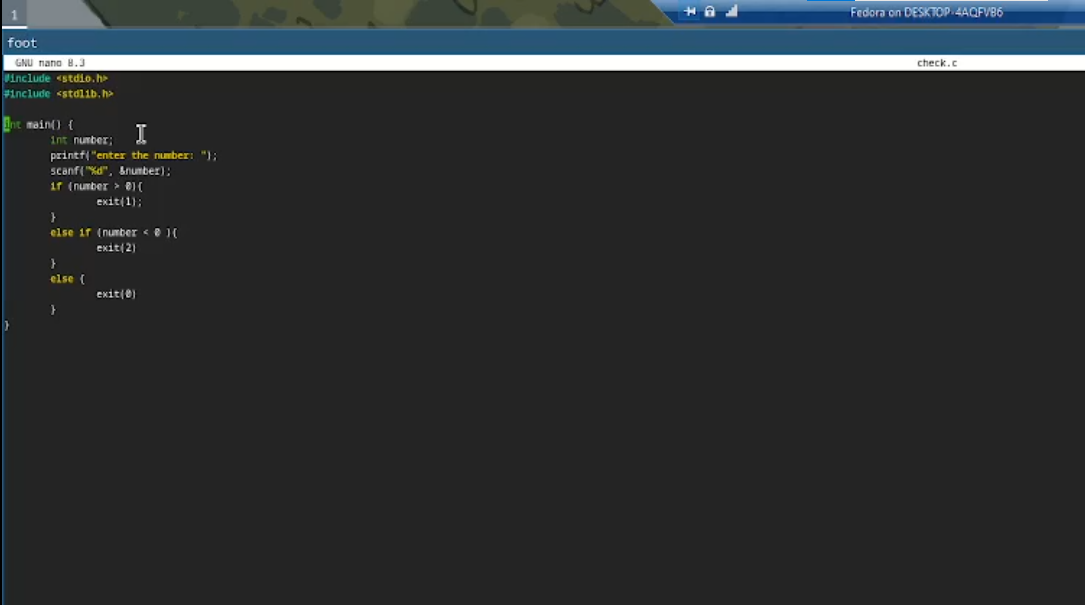
\includegraphics[width=0.7\linewidth,height=\textheight,keepaspectratio]{image/content1.png}

}

\caption{Содержимое скрипта 1}

\end{figure}%
\end{frame}

\begin{frame}{4.2 Содержимое скрипта 2}
\phantomsection\label{ux441ux43eux434ux435ux440ux436ux438ux43cux43eux435-ux441ux43aux440ux438ux43fux442ux430-2}
\begin{figure}[H]

{\centering 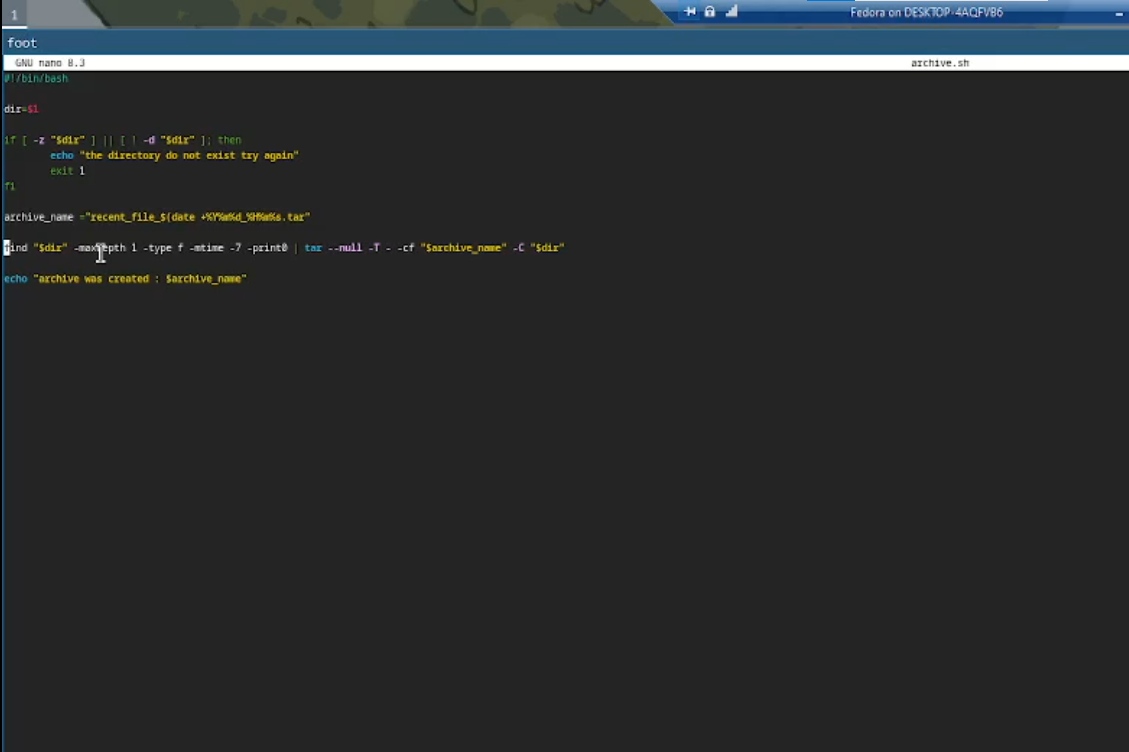
\includegraphics[width=0.7\linewidth,height=\textheight,keepaspectratio]{image/content2.png}

}

\caption{Содержимое скрипта 2}

\end{figure}%
\end{frame}

\begin{frame}{4.3 Содержимое shell скрипта}
\phantomsection\label{ux441ux43eux434ux435ux440ux436ux438ux43cux43eux435-shell-ux441ux43aux440ux438ux43fux442ux430}
\begin{figure}[H]

{\centering 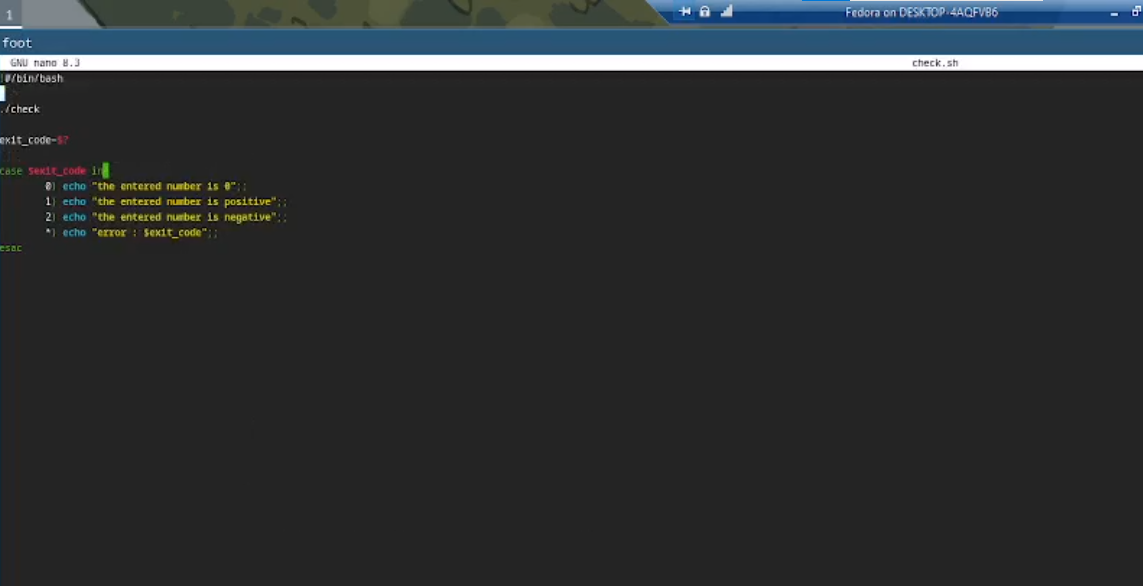
\includegraphics[width=0.7\linewidth,height=\textheight,keepaspectratio]{image/shcontent1.png}

}

\caption{Содержимое shell скрипта}

\end{figure}%
\end{frame}

\begin{frame}{4.4 Программный код}
\phantomsection\label{ux43fux440ux43eux433ux440ux430ux43cux43cux43dux44bux439-ux43aux43eux434}
\begin{figure}[H]

{\centering 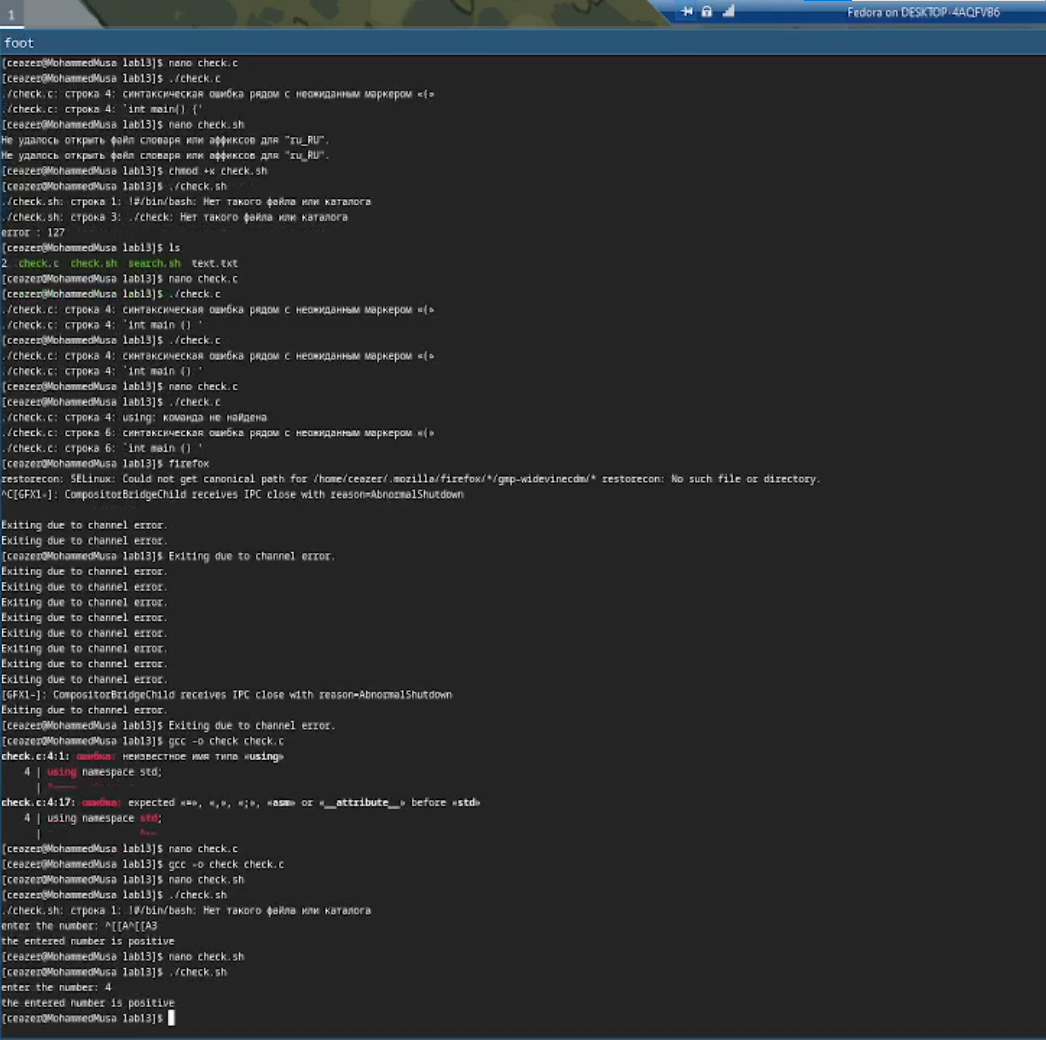
\includegraphics[width=0.7\linewidth,height=\textheight,keepaspectratio]{image/program1.png}

}

\caption{Программный код}

\end{figure}%
\end{frame}

\begin{frame}{4.5 Запуск программ}
\phantomsection\label{ux437ux430ux43fux443ux441ux43a-ux43fux440ux43eux433ux440ux430ux43cux43c}
\begin{figure}[H]

{\centering 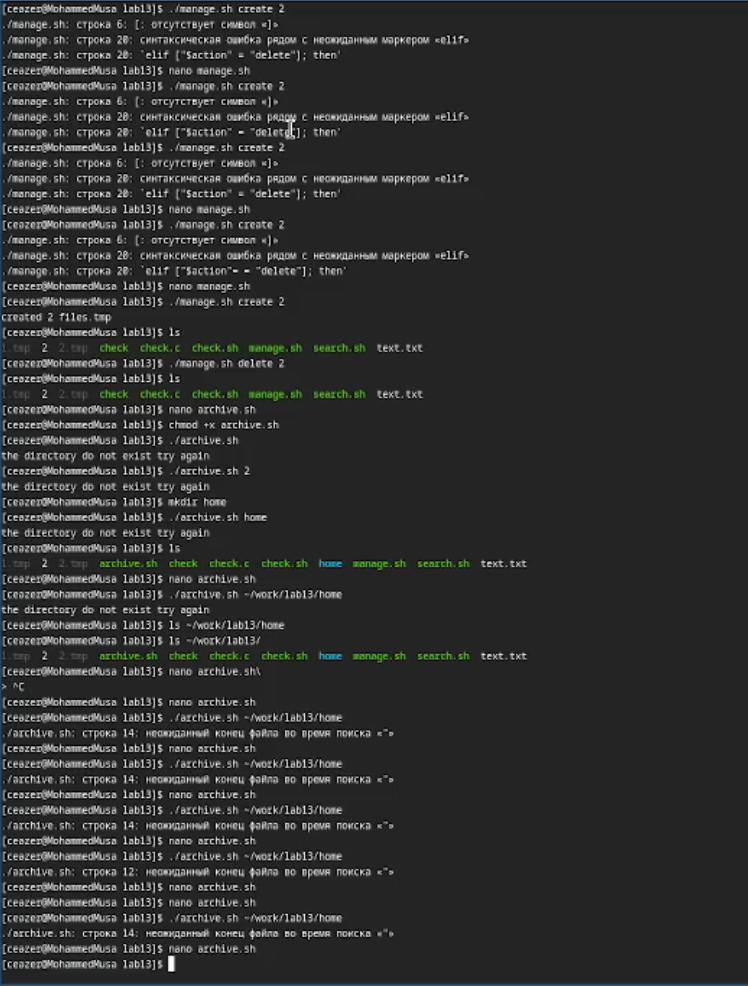
\includegraphics[width=0.7\linewidth,height=\textheight,keepaspectratio]{image/run2.png}

}

\caption{Запуск программ}

\end{figure}%
\end{frame}

\begin{frame}{4.6 Практические примеры}
\phantomsection\label{ux43fux440ux430ux43aux442ux438ux447ux435ux441ux43aux438ux435-ux43fux440ux438ux43cux435ux440ux44b}
Были созданы скрипты:

\begin{itemize}[<+->]
\tightlist
\item
  Скрипт приветствия с учетом времени
\item
  Скрипт обработки файлов с циклами
\item
  Калькулятор с функциями
\item
  Скрипт с обработкой опций
\item
  Интерактивное меню
\end{itemize}
\end{frame}

\begin{frame}[fragile]{4.7 Скрипт с переменными}
\phantomsection\label{ux441ux43aux440ux438ux43fux442-ux441-ux43fux435ux440ux435ux43cux435ux43dux43dux44bux43cux438}
\begin{Shaded}
\begin{Highlighting}[]
\CommentTok{\#!/bin/bash}
\VariableTok{name}\OperatorTok{=}\VariableTok{$1}
\VariableTok{current\_hour}\OperatorTok{=}\VariableTok{$(}\FunctionTok{date}\NormalTok{ +\%H}\VariableTok{)}

\BuiltInTok{echo} \StringTok{"Привет, }\VariableTok{$name}\StringTok{!"}

\ControlFlowTok{if} \BuiltInTok{[} \VariableTok{$current\_hour} \OtherTok{{-}lt}\NormalTok{ 12 }\BuiltInTok{]}\KeywordTok{;} \ControlFlowTok{then}
    \BuiltInTok{echo} \StringTok{"Доброе утро!"}
\ControlFlowTok{elif} \BuiltInTok{[} \VariableTok{$current\_hour} \OtherTok{{-}lt}\NormalTok{ 18 }\BuiltInTok{]}\KeywordTok{;} \ControlFlowTok{then}
    \BuiltInTok{echo} \StringTok{"Добрый день!"}
\ControlFlowTok{else}
    \BuiltInTok{echo} \StringTok{"Добрый вечер!"}
\ControlFlowTok{fi}
\end{Highlighting}
\end{Shaded}
\end{frame}

\begin{frame}[fragile]{4.8 Скрипт с циклами}
\phantomsection\label{ux441ux43aux440ux438ux43fux442-ux441-ux446ux438ux43aux43bux430ux43cux438}
\begin{Shaded}
\begin{Highlighting}[]
\CommentTok{\#!/bin/bash}
\VariableTok{count}\OperatorTok{=}\NormalTok{0}

\ControlFlowTok{for}\NormalTok{ file }\KeywordTok{in} \PreprocessorTok{*}\NormalTok{.txt}\KeywordTok{;} \ControlFlowTok{do}
    \KeywordTok{((}\VariableTok{count}\OperatorTok{++}\KeywordTok{))}
    \BuiltInTok{echo} \StringTok{"[}\VariableTok{$count}\StringTok{] Файл: }\VariableTok{$file}\StringTok{"}
    \BuiltInTok{echo} \StringTok{"    Строк: }\VariableTok{$(}\FunctionTok{wc} \AttributeTok{{-}l} \OperatorTok{\textless{}} \StringTok{"}\VariableTok{$file}\StringTok{"}\VariableTok{)}\StringTok{"}
    \BuiltInTok{echo} \StringTok{"    Слов: }\VariableTok{$(}\FunctionTok{wc} \AttributeTok{{-}w} \OperatorTok{\textless{}} \StringTok{"}\VariableTok{$file}\StringTok{"}\VariableTok{)}\StringTok{"}
\ControlFlowTok{done}

\BuiltInTok{echo} \StringTok{"Всего файлов: }\VariableTok{$count}\StringTok{"}
\end{Highlighting}
\end{Shaded}
\end{frame}

\begin{frame}[fragile]{4.9 Скрипт с функциями}
\phantomsection\label{ux441ux43aux440ux438ux43fux442-ux441-ux444ux443ux43dux43aux446ux438ux44fux43cux438}
\begin{Shaded}
\begin{Highlighting}[]
\CommentTok{\#!/bin/bash}

\FunctionTok{add()} \KeywordTok{\{}
    \BuiltInTok{echo} \VariableTok{$(($1} \OperatorTok{+} \VariableTok{$2))}
\KeywordTok{\}}

\FunctionTok{multiply()} \KeywordTok{\{}
    \BuiltInTok{echo} \VariableTok{$(($1} \OperatorTok{*} \VariableTok{$2))}
\KeywordTok{\}}

\BuiltInTok{echo} \StringTok{"10 + 5 = }\VariableTok{$(}\ExtensionTok{add}\NormalTok{ 10 5}\VariableTok{)}\StringTok{"}
\BuiltInTok{echo} \StringTok{"10 * 5 = }\VariableTok{$(}\ExtensionTok{multiply}\NormalTok{ 10 5}\VariableTok{)}\StringTok{"}
\end{Highlighting}
\end{Shaded}
\end{frame}

\section{5. Результаты}\label{ux440ux435ux437ux443ux43bux44cux442ux430ux442ux44b}

\begin{frame}{5.1 Выполненные задачи (1)}
\phantomsection\label{ux432ux44bux43fux43eux43bux43dux435ux43dux43dux44bux435-ux437ux430ux434ux430ux447ux438-1}
\begin{itemize}[<+->]
\tightlist
\item
  ✅ \textbf{Освоено создание shell скриптов}

  \begin{itemize}[<+->]
  \tightlist
  \item
    Структура с shebang
  \item
    Создание исполняемых файлов
  \item
    Различные способы запуска
  \end{itemize}
\end{itemize}
\end{frame}

\begin{frame}{5.2 Выполненные задачи (2)}
\phantomsection\label{ux432ux44bux43fux43eux43bux43dux435ux43dux43dux44bux435-ux437ux430ux434ux430ux447ux438-2}
\begin{itemize}[<+->]
\tightlist
\item
  ✅ \textbf{Изучена работа с переменными}

  \begin{itemize}[<+->]
  \tightlist
  \item
    Объявление и использование
  \item
    Специальные переменные
  \item
    Переменные окружения
  \item
    Операции с переменными
  \end{itemize}
\end{itemize}
\end{frame}

\begin{frame}{5.3 Выполненные задачи (3)}
\phantomsection\label{ux432ux44bux43fux43eux43bux43dux435ux43dux43dux44bux435-ux437ux430ux434ux430ux447ux438-3}
\begin{itemize}[<+->]
\tightlist
\item
  ✅ \textbf{Практикованы условные операторы}

  \begin{itemize}[<+->]
  \tightlist
  \item
    Оператор if-elif-else
  \item
    Операторы сравнения
  \item
    Логические операторы
  \item
    Оператор case
  \end{itemize}
\end{itemize}
\end{frame}

\begin{frame}{5.4 Выполненные задачи (4)}
\phantomsection\label{ux432ux44bux43fux43eux43bux43dux435ux43dux43dux44bux435-ux437ux430ux434ux430ux447ux438-4}
\begin{itemize}[<+->]
\tightlist
\item
  ✅ \textbf{Освоены циклы}

  \begin{itemize}[<+->]
  \tightlist
  \item
    Цикл for (диапазоны, файлы)
  \item
    Цикл while
  \item
    Цикл until
  \item
    Команды break и continue
  \end{itemize}
\end{itemize}
\end{frame}

\begin{frame}{5.5 Выполненные задачи (5)}
\phantomsection\label{ux432ux44bux43fux43eux43bux43dux435ux43dux43dux44bux435-ux437ux430ux434ux430ux447ux438-5}
\begin{itemize}[<+->]
\tightlist
\item
  ✅ \textbf{Изучена отладка скриптов}

  \begin{itemize}[<+->]
  \tightlist
  \item
    Опции bash (-x, -v, -n)
  \item
    Команды set
  \item
    Отладочные сообщения
  \item
    Проверка синтаксиса
  \end{itemize}
\end{itemize}
\end{frame}

\begin{frame}{5.6 Дополнительные навыки}
\phantomsection\label{ux434ux43eux43fux43eux43bux43dux438ux442ux435ux43bux44cux43dux44bux435-ux43dux430ux432ux44bux43aux438}
\begin{itemize}[<+->]
\tightlist
\item
  ✅ Создание функций с параметрами
\item
  ✅ Работа с файлами
\item
  ✅ Интерактивные скрипты
\item
  ✅ Обработка текста
\item
  ✅ Управление потоками
\item
  ✅ Организация кода
\end{itemize}
\end{frame}

\begin{frame}{5.7 Полученные знания}
\phantomsection\label{ux43fux43eux43bux443ux447ux435ux43dux43dux44bux435-ux437ux43dux430ux43dux438ux44f}
\textbf{Освоены:}

\begin{itemize}[<+->]
\tightlist
\item
  \textbf{Основы bash} --- синтаксис, структура, выполнение
\item
  \textbf{Переменные} --- типы, операции, окружение
\item
  \textbf{Управляющие конструкции} --- условия, циклы
\item
  \textbf{Функции} --- создание, параметры, возврат
\item
  \textbf{Отладка} --- методы, инструменты, оптимизация
\end{itemize}
\end{frame}

\section{6. Заключение}\label{ux437ux430ux43aux43bux44eux447ux435ux43dux438ux435}

\begin{frame}{6.1 Выводы}
\phantomsection\label{ux432ux44bux432ux43eux434ux44b}
\begin{itemize}[<+->]
\tightlist
\item
  Освоены основы shell программирования
\item
  Изучены переменные, условия, циклы и функции
\item
  Практикована обработка аргументов
\item
  Освоены методы отладки скриптов
\item
  Получены навыки автоматизации задач
\end{itemize}
\end{frame}

\begin{frame}{6.2 Практическое применение}
\phantomsection\label{ux43fux440ux430ux43aux442ux438ux447ux435ux441ux43aux43eux435-ux43fux440ux438ux43cux435ux43dux435ux43dux438ux435}
\begin{itemize}[<+->]
\tightlist
\item
  \textbf{Автоматизация} --- рутинные операции
\item
  \textbf{Системное администрирование} --- управление системой
\item
  \textbf{DevOps} --- CI/CD, развертывание
\item
  \textbf{Обработка данных} --- парсинг, отчеты
\item
  \textbf{Разработка инструментов} --- утилиты CLI
\end{itemize}
\end{frame}

\begin{frame}{6.3 Значимость навыков}
\phantomsection\label{ux437ux43dux430ux447ux438ux43cux43eux441ux442ux44c-ux43dux430ux432ux44bux43aux43eux432}
Полученные навыки являются \textbf{фундаментальными} для:

\begin{itemize}[<+->]
\tightlist
\item
  Эффективной работы в Linux
\item
  Автоматизации задач
\item
  Системного администрирования
\item
  Разработки ПО
\item
  DevOps практик
\end{itemize}
\end{frame}

\begin{frame}[standout]{6.4 }
\phantomsection\label{section}
Спасибо за внимание!

Вопросы?
\end{frame}




\end{document}
